\chapter{Generation of design idea using Dall-E}
\label{chatgpt-prompts}

DALL-E was instrumental in generating the design concept for a future Smart Patch. Multiple prompts were used to iteratively refine the final design output. \\

\noindent \textbf{Prompts}\\
\begin{enumerate}
    \item Create an image of an IoT device that doesn't resemble a smartwatch.
    \item Show a device that can be easily worn on the body and conveys a sense of health and wellness.
    \item It should be compact, roughly the same size as a smartwatch, but distinctly different.
    \item Make it resemble an earphone-like accessory, rather than a smartwatch.
    \item It shouldn't have a microphone or speaker.
    \item It should sit behind the ear.
\end{enumerate}

The final output image, shown in Figure \ref{fig:dall-e-generated-image}, reflects these prompts.

\begin{figure}
    \centering
    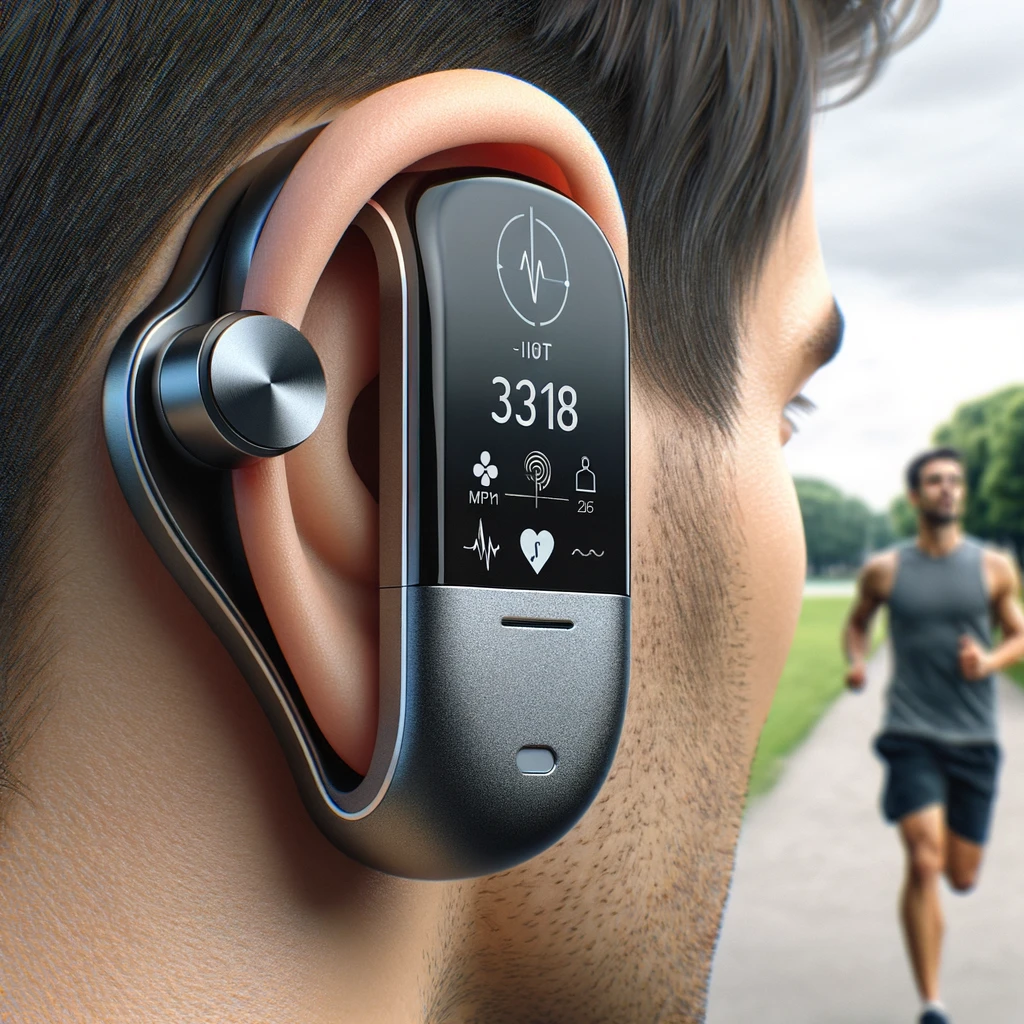
\includegraphics[width=1\linewidth]{images/image-chatgpt.png}
    \caption{Dall-E generated image}
    \label{fig:dall-e generated image}
\end{figure}


Subsequently, the background was removed, and a plain blue box was placed behind the image, with the label "Generated using DALL-E."

